\subsection{DAC Control} \label{subsec:DAC_CONTROL} 
Section \refq{ch:SysArchitecture} shows that the the Sample Controller is responsible for controlling the DAC such that a stable sine wave is generated. The logic responsible for this will be described in this section. The specific section of the Sample Controller that handles the DAC logic is referred to as the DAC Control. A block diagram of the DAC Control can be seen on figure \refq{fig:7_2_3_DAC_CONTROL}.

\begin{figure}[H]
    \centering
    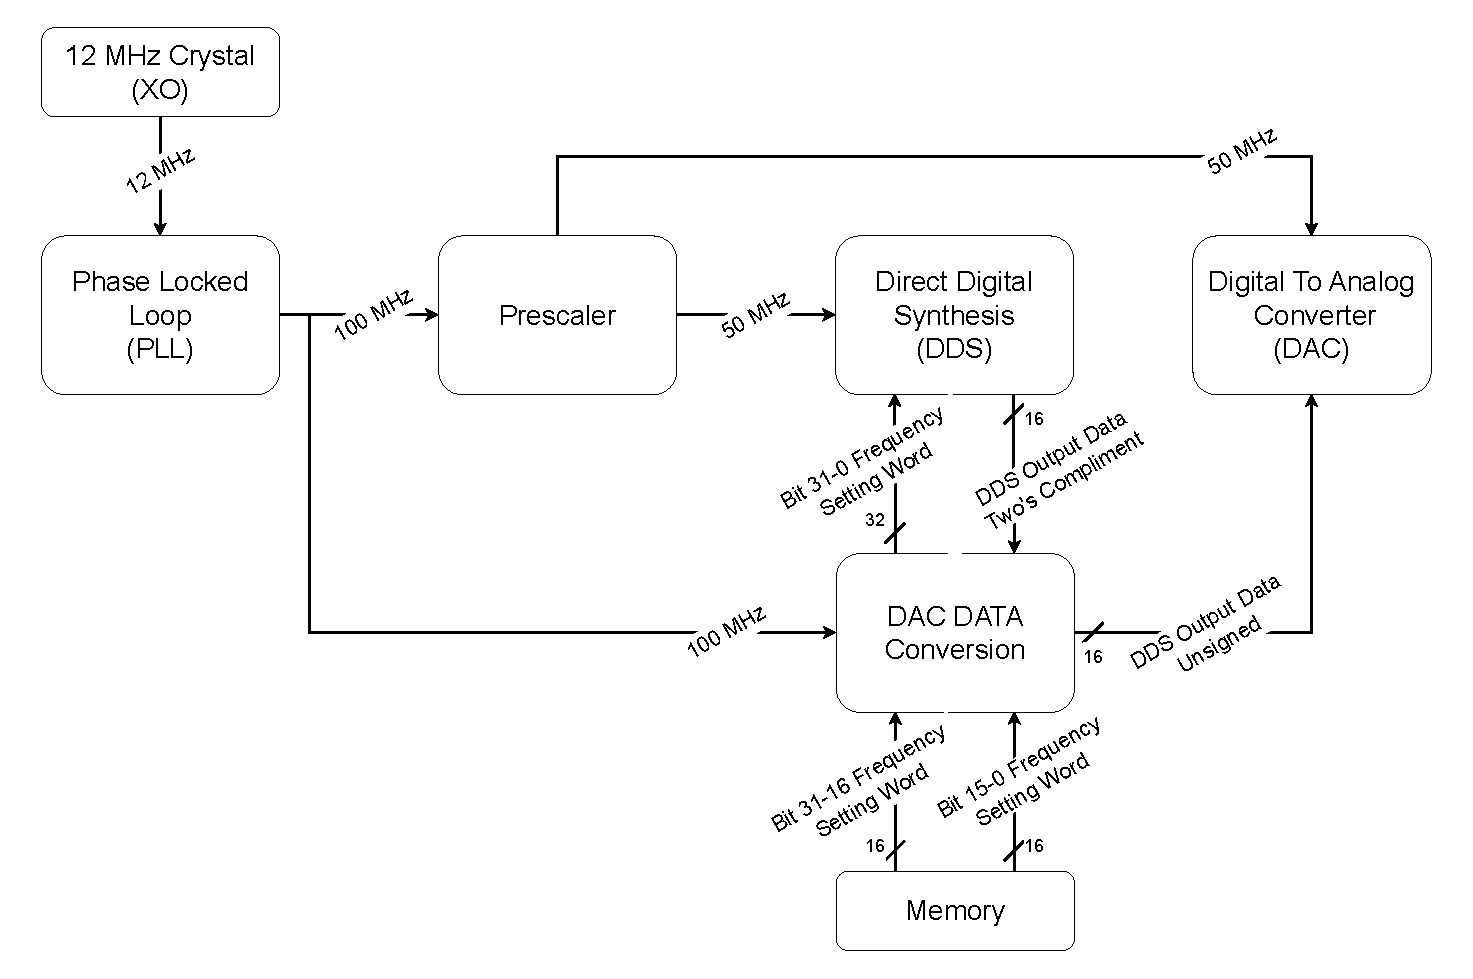
\includegraphics[clip, trim=0 0 0 0, width=1\textwidth]{Sections/7_SystemDesign/Figures/7_2_3_DAC_CONTROL.pdf}
    \caption{Block diagram of the DAC Control logic, the DAC is on the Analog Front End, it is shown here for completeness.}
    \label{fig:7_2_3_DAC_CONTROL}
\end{figure}

There are numerous of ways to generate sine waves, for this project a digital implementation has been favored due to the precise resolution that it offers. Requirement §1 from section \refq{ch:SystemRequirements} states that the frequency resolution must be at least \SIQ{1}{\hertz}. To achieve this, a Direct Digital Synthesis (DDS) principle has implemented. This essentially allows for a frequency resolution that is the DAC update rate divided by the length of the frequency setting word \cite{Fundamentals_DDS}. With a 32 bit wide frequency setting word, as specified by requirement §6.3.13 in section \refq{subsec:SampleControlSpec}, the resulting frequency resolution would be $f_{res} = \frac{DAC_{CLK}}{2^{32}}$.

The used DAC is an LTC1668, capable of an update rate of \SIQ{50}{\mega\hertz}. This essentially allows for a frequency resolution of \SIQ{11.6415}{\milli\hertz}, see equation \refq{eq:7_2_3_resolution}, assuming an update rate of \SIQ{50}{\mega\hertz}.

\begin{equation}
    \label{eq:7_2_3_resolution}
    f_{res} = \frac{\SIQ{50}{\mega\hertz}}{2^{32}} \Rightarrow \SIQ{11.6415}{\milli\hertz}. 
\end{equation}

Xilinx offers a complete "drag and drop" DDS block. The project team has settled on using this as it supports DAC resolutions of up to 18 bits and frequency setting words up to 48 bits, essentially making it ideal for the required DAC Control block. The principle of Direct Digital Synthesis will not be explained in this document, as it is not part of the scope of the project.

The DDS block is configured to take in a 32 bit wide frequency setting word, a \SIQ{50}{\mega\hertz} clock, and a frequency update signal. The output of the DDS block is configured for a 16 bit wide sine approximation as two's compliment.

All other blocks than the DDS shown in figure \refq{fig:7_2_3_DAC_CONTROL} are essentially there to "support" the DDS block. A \SIQ{50}{\mega\hertz} clock is generated via a Phase Locked Loop (PLL) and a prescaler. The PLL outputs a \SIQ{100}{\mega\hertz} signal that is divided by two and fed to the DDS block. The prescaler will also generate a \SIQ{50}{\mega\hertz} pulse train that is delayed from the DDS clock signal. This delayed pulse train is used to update the DAC.

The 16 bit wide output data of the DDS contains an approximated full-scale sine wave in two's compliment. The DAC however requires unsigned values as an input, and thus the DDS output data must be converted to a 16 bit wide unsigned bus. Furthermore the memory holds data in 16 bit registers, meaning that the 32 bit frequency setting word must be two registers that are concatenated. The DAC DATA Conversion block handles this concatenation and conversion from two's compliment to unsigned.





